\section{Experimental Setup}
\label{sec:experimentalSetup}

We use trace based simulation to compare alternative implementations
of applications that perform continuous sensing.  We consider
approaches that assume that the phone is always-on, performs duty
cycling, has access to hardware that buffers sensor readings, provides
an API that either lets applications register for notifications based
on pre-defined activity recognition, and provides an API that lets
applications specify custom wakeup conditions by configuring
pre-defined filters.

The rest of this section describes our trace
collection methodology, the sensing applications we implemented, and
the operation of our trace-based simulator.

\subsection{Trace Collection}

Annotating accelerometer traces collected from human subjects with
ground truth information about the performed actions is both extremely
time-consuming and prone to errors.  Instead, to collect the
accelerometer traces for our experiments we used an AIBO ERA 210 robot
(Figure \ref{fig:aibo}). The robot would perform a course consisting
of a sequence of actions and record timestamps for the beginning and
end of each action. The set of performed actions and timestamps were
outputted to a log file and represent the {\em ground truth} for our
simulation-based experiments.  To record the accelerometer trace, we
attached a Google Nexus 4 to the back of the dog and ran an
application that collected accelerometer readings while the robot
completed the course.

To eliminate bias, the courses we asked the robot to complete were
randomly generated.  Each course consisted of five different actions:
standing idle, walking, seat-to-stand transition, stand-to-seat
transition, and headbut.  To cover a range of activity levels, we
divided our course into three different groups.  Courses in groups 1, 2
and 3 spent 90\%, 50\% and 10\% of the time standing idle,
respectively.  The reminder of the time was allocated as follows: 90\%
for walking, 9\% for transitions between seating and standing, and 1\%
for headbuts.  This setups allows us to experiment with detecting
actions that are very common, somewhat frequent, and very rare.
Figure \ref{fig:actionTimes} shows the average amount of time each
action is being perform for the traces in each group, as a percentage
of the average trace length.  {\em TODO: mention how many courses from
  each group we ran}





\begin{figure}[t]
	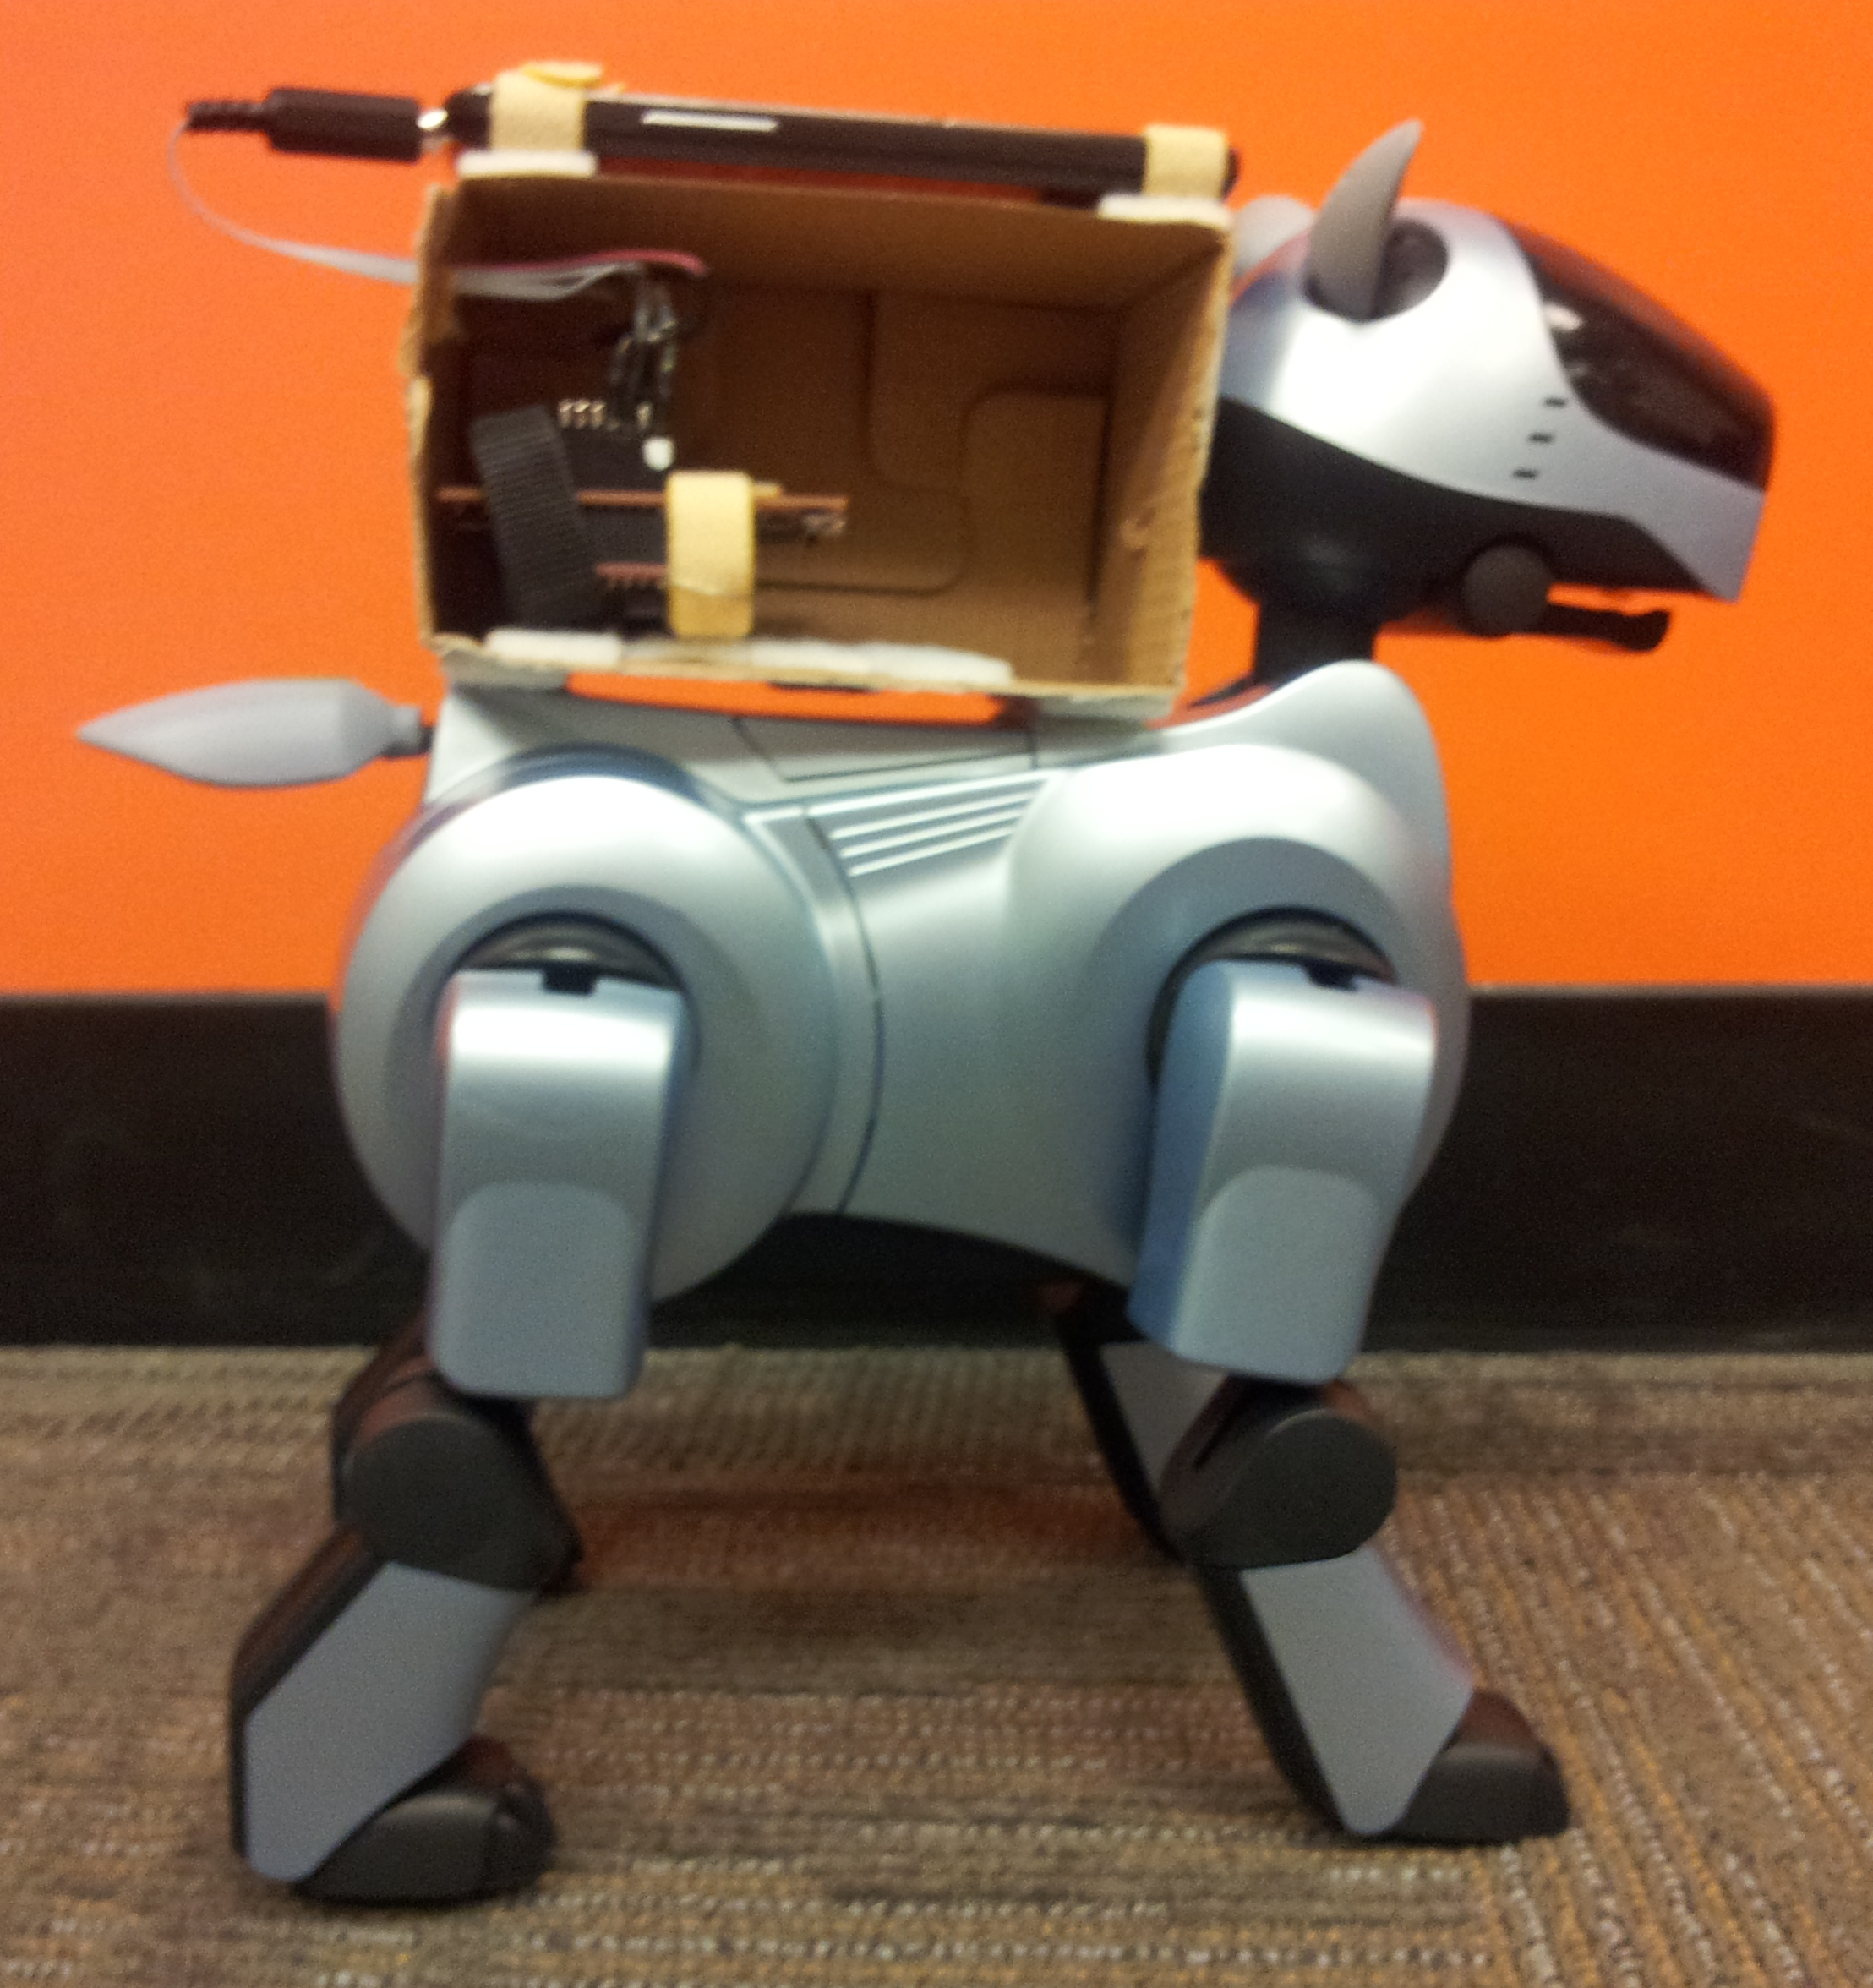
\includegraphics[width=8.5cm]{aibo_ers_210.jpg}
	\caption{AIBO ERS 210 robot used to collect the accelerometer traces}
	\label{fig:aibo}
\end{figure}


\begin{figure}[t]
	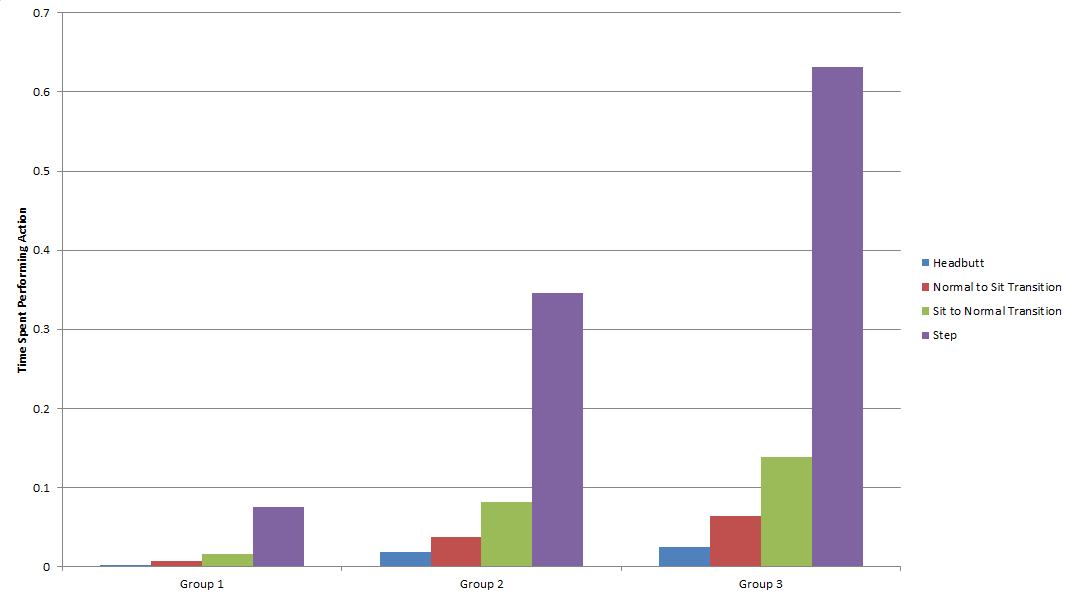
\includegraphics[width=8.5cm]{action_times.png}
	\caption{Time spent performing actions of specific types as a percentage or trace length}
	\label{fig:actionTimes}
\end{figure}


\subsection{Applications}

We implemented 3 applications:

\begin{itemize}

\item {\bf Steps} counts how many steps the dog takes when it walks by
  looking for local maxima on the x-axis.


\item {\bf Stand-seat} detects transitions between seating and
  standing  by monitoring changes in the acceleration due to gravity
  on the y and z axes.



\item {\bf Headbut} detects a headbut motion by searching for local
  minima on the y-axis.

\end{itemize}

We developed two versions of each application.  Experiments that
evaluate always-on operation, duty-cycling, and buffering, use
single-stage versions of the applications that perform activity
recognition by running on the phone sets of low-pass filters based on
Fast-Fourier Transformations.  Experiments that evaluate the use of
wakeup conditions have an additional stage that runs on the low-power
sensor board, and implements either a simple threshold, an exponential
average or FFT.  The low power processor wakes up the phone only when
it believes that an event of interest has been detected.  The
application then runs an additional FFT on the phone to eliminate any
false positives, (events that where missidentified by the low-power
processor).


Additionally, the Always Awake simulations show
the accuracy of the implemented applications in terms of event of
interest detection precision and recall. 


Figure \ref{fig:aaRecallByGroup} shows the average recall for all
applications when executing on a phone that is kept always-on.  With
the exception of the headbutt action in Group 1, event recall is above
95\% for all actions and groups. The headbutt action in Group 1
appears to be an outlier because Group 1 contains traces with the
least amount of actions and headbutts are the scarcest actions,
occurring only about once per trace. Figure
\ref{fig:aaPrecisionByGroup2} shows the detection precision of each of
the events of interest averaged over the traces in each group. For all
cases, the applications achieved a detection precision above 82\%.



\begin{figure}[t]
	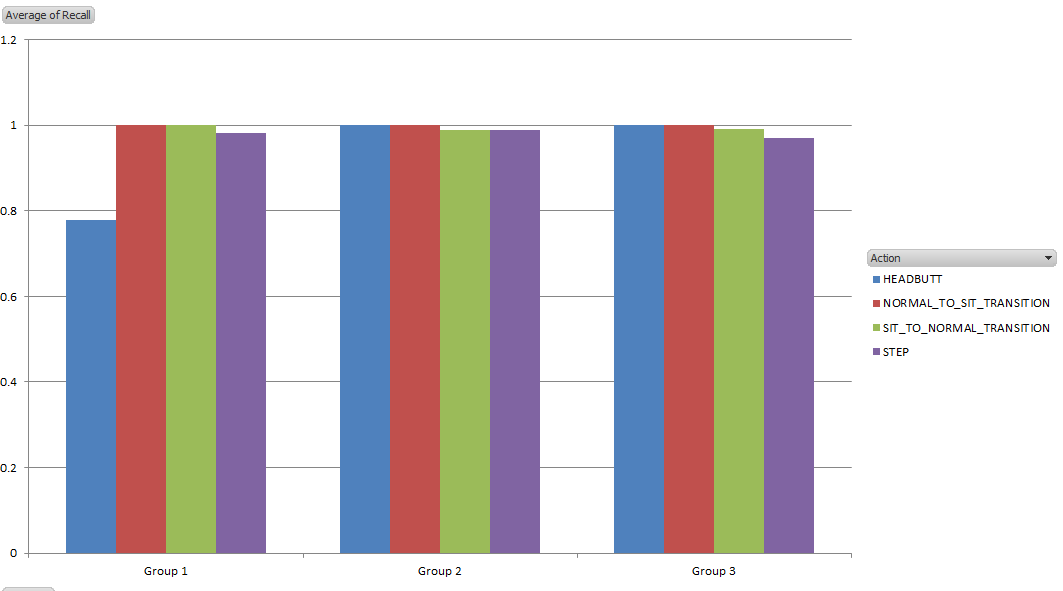
\includegraphics[width=8.5cm]{aa_recall_by_group.png}
	\caption{Always Awake: Recall by Group}
    	\label{fig:aaRecallByGroup}
\end{figure}


\begin{figure}[t]
	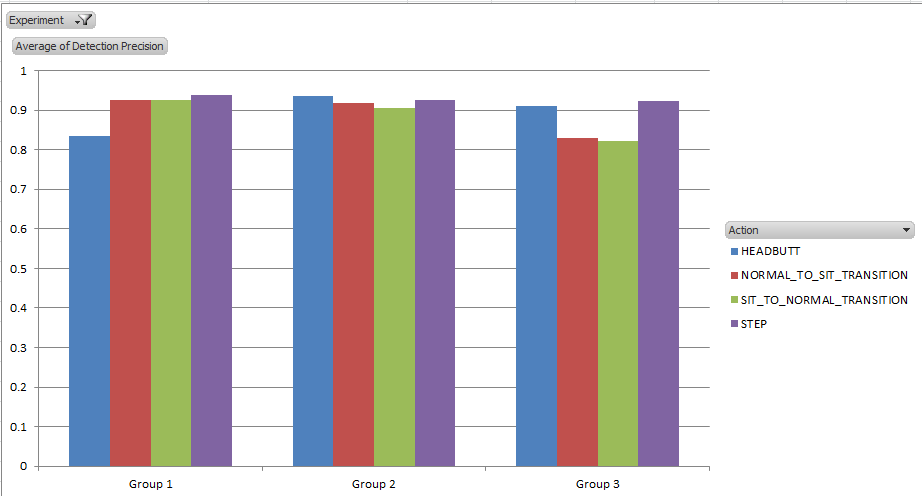
\includegraphics[width=8.5cm]{aa_precision_by_group2.png}
	\caption{Always Awake: Detection Precision by Group}
    	\label{fig:aaPrecisionByGroup}
\end{figure}


\subsection{Trace-based Simulator}

Each collected accelerometer trace is an ordered set of accelerometer
readings. Each reading contains the x-, y- and z-components of the
acceleration vector and a timestamp indicating when the reading was
produced.

The simulator processes the readings one at a time, similarly to how a
mobile device would receive accelerometer readings in real-time, as
they are produced by the sensor. Based on the wake-up approach, the
simulator determines which of the readings would cause the device to
wake-up. Also, the simulator determines what readings need to be sent
to the running applications. At the end of the run, the simulator
outputs the following metrics:

\begin{enumerate}
\setlength{\itemsep}{-3pt}  

\item Amount of time the device would have been awake.

\item Total number of device wake-up.

\item Number of wake-ups that did not result in an event of interest
  being detected by the application.

\item True positives, false positives and false negatives for each event of interest.

\item Recall and precision for each event of interest

\item Power consumption over the duration of the trace.   This value is derived from the 
  energy measurements presented in section \ref{sec:prototype}, the
  amount of time the device is awake, the amount of time it is asleep
  and the number of transitions between the two states.

\end{enumerate}


\subsection{Discussion}

Since we are mainly interested in actions that would normally be
performed by humans, we tried to configure the robot to perform
actions with similar acceleration signatures.  Robot walking has a
similar acceleration signature as its human counterpart, though at a
much lower intensity.  The headbutts are meant to represent very
infrequent human actions such as falling. We found that robot stance
transitions between the normal and sitting postures are very similar
in their acceleration signature as humans sitting down and standing
up.


The use of a robot could have enabled us to run live experiments
because performing the same sequence of actions multiple times would
result in similar accelerometer traces. We opted not to do so for
several reasons. Each run takes upwards of an hour to execute. Our
goal was to obtain results for a multitude of wake-up approaches, each
under multiple parameter configurations. The combination of all
courses and wake-up configurations would have required over a year of
continuous live experimentation. Running trace-based simulations
allows us to perform an exhaustive exploration of the parameter
configuration space. Moreover, taking fine grain power consumption
measurements while the robot is in motion is not trivial.
Nonetheless, this is part of our future work.


